%\documentclass[a4paper,twocolumn]{article}
\documentclass[a4paper,10pt]{article}

%\usepackage{fancyhdr}
%\usepackage{anysize}
%\usepackage{pslatex}
\usepackage{fullpage}
\usepackage{amsmath,amssymb,amsthm}
\usepackage{undertilde}
\usepackage{epsfig}
\usepackage[small,ruled]{caption}
\usepackage{subfig}
\usepackage{multirow}
\usepackage{lscape}
\usepackage{listings}
\usepackage{float}
\usepackage[nothing]{algorithm}
\usepackage{algorithmic}
\usepackage{paralist}
\setdefaultenum{1)}{(a)}{i)}{A)}
\usepackage{graphicx}
\usepackage{url}
\usepackage{longtable}
%\usepackage{xtab}
\usepackage{tikz}
\usetikzlibrary{arrows,shapes,matrix,patterns}
\usepackage{hyperref}
\usepackage{xspace}

\newcommand{\GROOVE}{\textrm{Groove}\xspace}
\newcommand{\NAUTY}{\texttt{nauty}\xspace}
\newcommand{\BLISS}{\texttt{bliss}\xspace}
\newcommand{\SAUCY}{\texttt{saucy}\xspace}

\tikzstyle{vertex} = [circle,draw,minimum size=20pt,inner sep=0pt]
\tikzstyle{edge} = [draw,thick,->,bend right]
\tikzstyle{node} = [rectangle,draw,minimum width=20pt,inner sep=4pt]
\tikzstyle{point} = [circle,draw,fill,minimum size=5pt,inner sep=0pt,outer sep=0pt]

\algsetup{linenosize=\scriptsize}

\title{
  Graphs
}
%\author{Gijs Kant\\kant@cs.utwente.nl}

\begin{document}
\maketitle

\begin{figure}[tph]
\centering
\subfloat[Size.]{\label{fig:size:unflagged-platoon}
    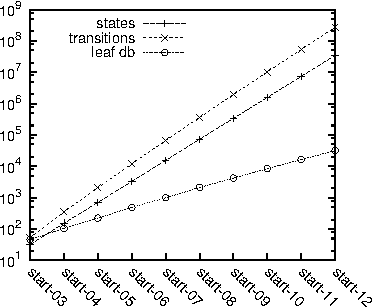
\includegraphics[width=2.5in]{../graphs/size_unflagged-platoon.pdf}
 }
\quad
\subfloat[Memory.]{\label{fig:memory:unflagged-platoon}
   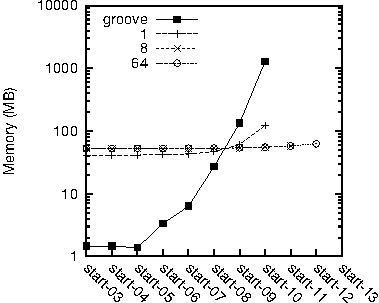
\includegraphics[width=2.5in]{../graphs/mem_unflagged-platoon.pdf}
 }
\\
  \subfloat[Time.]{\label{fig:results:unflagged-platoon}
    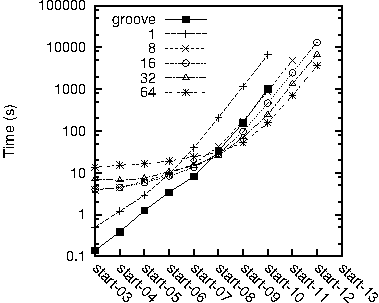
\includegraphics[width=2.5in]{../graphs/results_unflagged-platoon.pdf}
  }
\quad
 \subfloat[Speedup.]{\label{fig:speedup:unflagged-platoon}
    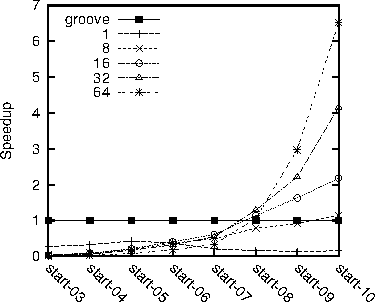
\includegraphics[width=2.5in]{../graphs/results_unflagged-platoon_speedup.pdf}
  }
 \caption{\texttt{unflagged-platoon}.}
\label{fig:results-unflagged-platoon}
\end{figure}

\begin{figure}[tph]
\centering
\subfloat[\texttt{start-08}.]{\label{fig:stacked:unflagged-platoon-start-08}
   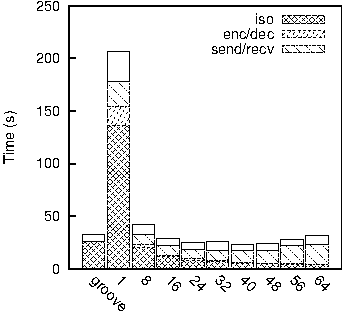
\includegraphics[width=2.5in]{../graphs/results_unflagged-platoon_start-08_stacked.pdf}
 }
\quad
 \subfloat[\texttt{start-08}.]{\label{fig:stacked:unflagged-platoon-start-08-wogrey}
    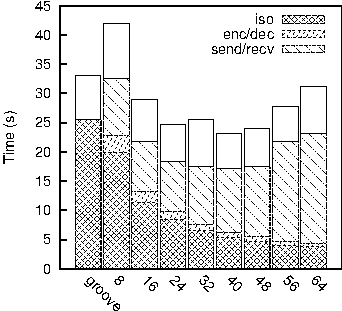
\includegraphics[width=2.5in]{../graphs/results_unflagged-platoon_start-08_stacked_wo_grey.pdf}
  }
\\
\subfloat[\texttt{start-10}.]{\label{fig:stacked:unflagged-platoon-start-10}
   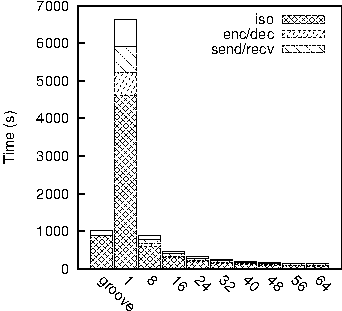
\includegraphics[width=2.5in]{../graphs/results_unflagged-platoon_start-10_stacked.pdf}
 }
\quad
 \subfloat[\texttt{start-10}.]{\label{fig:stacked:unflagged-platoon-start-10-wogrey}
   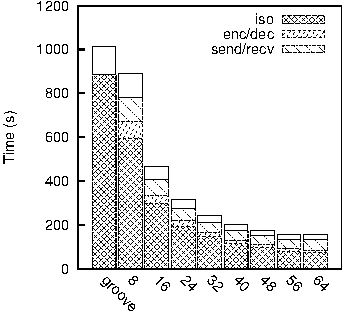
\includegraphics[width=2.5in]{../graphs/results_unflagged-platoon_start-10_stacked_wo_grey.pdf}
 }
 \\
\subfloat[\texttt{start-12}.]{\label{fig:stacked:unflagged-platoon-start-12}
   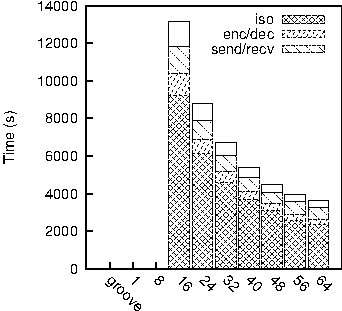
\includegraphics[width=2.5in]{../graphs/results_unflagged-platoon_start-12_stacked.pdf}
 }
 \caption{\texttt{unflagged-platoon}.}
\label{fig:results-unflagged-platoon-stacked}
\end{figure}

\end{document}
